\documentclass[11pt]{article}

\usepackage[margin=0.85in]{geometry}
\usepackage[utf8]{inputenc}
\usepackage[T1]{fontenc}
\usepackage{lmodern}
\usepackage{graphicx}
\usepackage{booktabs}
\usepackage{array}
\usepackage{xcolor}
\usepackage{hyperref}
\usepackage{enumitem}

\hypersetup{
  colorlinks=true,
  linkcolor=blue!45!black,
  urlcolor=blue!45!black
}

\setlength{\parindent}{0pt}
\setlength{\parskip}{0.55em}
\renewcommand{\arraystretch}{1.18}

\title{\textbf{Decision Variables for the Garrido SCRES-RL Paper}\\
\large Meeting note: Track B, post-CDC control, buffers, and KAN/CAN}
\author{Prepared for discussion with Prof. Garrido and David}
\date{3 July 2026}

\begin{document}
\maketitle

\section*{Purpose}

This note separates two decisions that were mixed together in the meeting:

\begin{enumerate}[leftmargin=1.5em]
  \item \textbf{Decision surface:} which supply-chain variables the agent is allowed to control.
  \item \textbf{Neural architecture:} whether the controller is PPO+MLP, recurrent PPO, DMLPA/CAN, or KAN.
\end{enumerate}

The current evidence says both must be decided in this order. First freeze a
physically defensible decision surface. Then run the neural architecture on that
surface. A stronger network cannot rescue a decision surface that violates
inventory conservation or does not reach the operational bottleneck.

\section*{Recommendation for the meeting}

\textbf{Recommended Paper 1 path:} keep the proven Track B decision surface as
the main paper lane. It has the strongest evidence, does not create inventory,
and already answers the central question: RL improves SCRES when the action
space reaches the downstream recovery bottleneck.

\textbf{Recommended Garrido extension:} if Prof. Garrido wants literal
post-CDC buffers, implement them as a \emph{conservative sidecar}: continuous
buffer targets are allowed, but replenishment must be a DES event constrained by
upstream inventory, capacity, lead time, and cost. Run a static/oracle gate
first; train CAN/KAN only if the gate shows real headroom.

\textbf{Architecture statement:} KAN/CAN deserves a real opportunity. Real-KAN
now improves Excel ReT over PPO+MLP in 10/10 matched seeds, but at much higher
utilization cost. This makes it a strong architecture sidecar and a direct
answer to Garrido's KAN concern, but not yet a replacement for the paper's
PPO+MLP spine.

\section*{Operations selected and why}

The selected operations follow the thesis topology and the meeting boundary
``from the Distribution Centre downward.'' Op3 is the CDC/WDC. The strict
post-CDC diagnostic freezes Op3 and leaves only downstream authority.

\begin{figure}[ht]
  \centering
  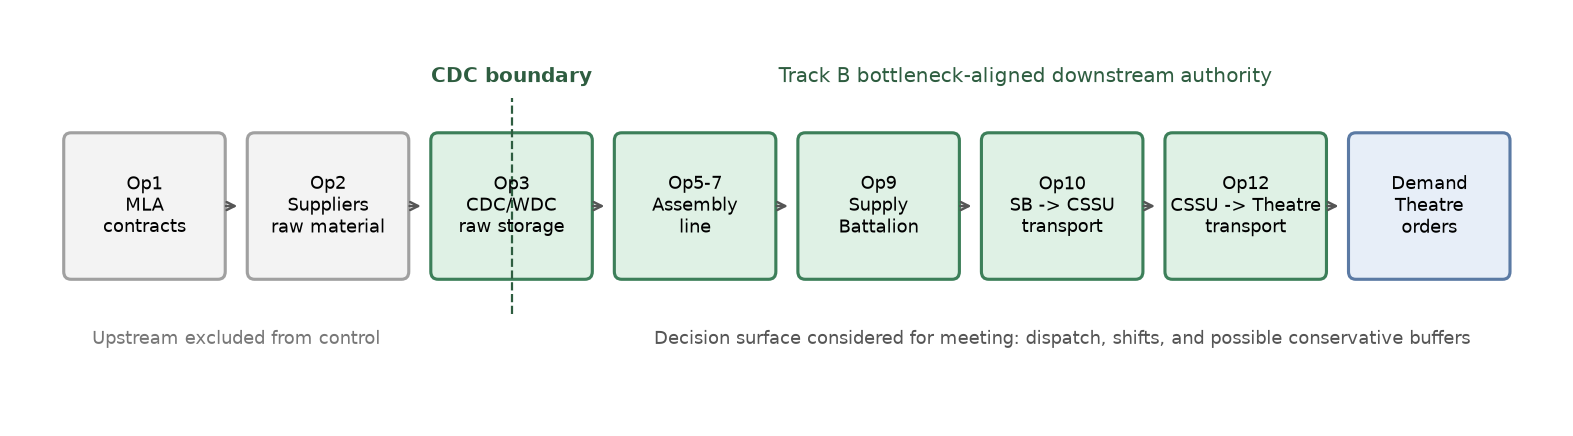
\includegraphics[width=\linewidth]{figures/fig1_topology_selected_operations.pdf}
  \caption{Selected operations in the Garrido-grounded supply-chain topology.}
\end{figure}

\begin{table}[ht]
\centering
\small
\begin{tabular}{p{0.12\linewidth}p{0.26\linewidth}p{0.27\linewidth}p{0.25\linewidth}}
\toprule
\textbf{Operation} & \textbf{Thesis role} & \textbf{Why selected} & \textbf{Decision variable} \\
\midrule
Op3 / CDC-WDC & Receives, verifies, and stores raw materials. & It is the meeting boundary: ``CDC downward.'' It also tests whether CDC authority is necessary. & In full Track B: raw-material dispatch quantity and reorder point. In strict post-CDC: frozen. \\
Op5-7 / Assembly & Converts raw materials into rations. & Determines recovery capacity when demand/backlog accumulates. & Shift level, implemented continuously and mapped to S1/S2/S3 thresholds. \\
Op9 / Supply Battalion & Stores and dispatches finished rations downstream. & First downstream ration buffer and dispatch point. & Dispatch quantity/reorder-point controls; candidate node for conservative buffer target. \\
Op10 / SB to CSSU & Transport leg from Supply Battalion to CSSUs. & One of the binding downstream recovery bottlenecks found empirically. & Dispatch multiplier for q-min/q-max. \\
Op12 / CSSU to Theatre & Final transport leg to theatre demand. & Second binding downstream recovery bottleneck; directly affects order recovery tails. & Dispatch multiplier for q-min/q-max. \\
\bottomrule
\end{tabular}
\caption{Decision nodes selected from the thesis topology.}
\end{table}

\section*{Alternative 1: Track B operational control}

This is the currently proven lane. It does not control supplier contracts or
upstream procurement. It controls CDC/downstream dispatch and assembly
capacity, with all material movements constrained by actual inventory.

\subsection*{Full Track B variables}

\begin{table}[ht]
\centering
\small
\begin{tabular}{p{0.18\linewidth}p{0.22\linewidth}p{0.48\linewidth}}
\toprule
\textbf{Variable} & \textbf{Node} & \textbf{Meaning} \\
\midrule
\texttt{op3\_q} & Op3 / CDC & Weekly raw-material dispatch quantity from CDC/WDC to assembly. \\
\texttt{op3\_rop} & Op3 / CDC & Reorder/dispatch timing at the CDC boundary. \\
\texttt{op9\_q} & Op9 & Supply Battalion dispatch quantity. \\
\texttt{op9\_rop} & Op9 & Supply Battalion dispatch timing. \\
\texttt{op5\_q} & Op5 & Present in the historical contract but currently inert unless an Op5 buffer is explicitly initialized; it is not load-bearing in Track B. \\
\texttt{shift} & Assembly & Continuous action mapped to S1/S2/S3 assembly shifts. \\
\texttt{op10\_q} & Op10 & Dispatch multiplier for the SB-to-CSSU transport leg. \\
\texttt{op12\_q} & Op12 & Dispatch multiplier for the CSSU-to-theatre transport leg. \\
\bottomrule
\end{tabular}
\caption{Full Track B action surface.}
\end{table}

\subsection*{Strict post-CDC variant}

The strict variant freezes Op3/CDC controls at the Garrido baseline and keeps
only downstream dispatch plus shift authority. This directly answers the
question: does the result depend on controlling the CDC? The answer is no.

\begin{itemize}[leftmargin=1.5em]
  \item PPO post-CDC-only Excel ReT: 0.005838.
  \item Best static comparator Excel ReT: 0.005428.
  \item Order-level ReT delta: +0.0003967.
  \item Seed signs: 5/5 positive; paired episode signs: 60/60 positive.
\end{itemize}

\section*{Alternative 2: conservative post-CDC buffers}

This is the literal version of Prof. Garrido's request: allow buffers in nodes
after the CDC. The important design rule is that the buffer cannot be filled by
magic. A continuous action is compatible with DES, but inventory conservation is
not optional.

\begin{figure}[ht]
  \centering
  \scriptsize
  \setlength{\fboxsep}{3pt}
  \makebox[\linewidth][c]{%
  \fbox{\parbox[c][0.62cm][c]{0.105\linewidth}{\centering Upstream\\inventory}}
  \hspace{0.01\linewidth}$\rightarrow$\hspace{0.01\linewidth}
  \fbox{\parbox[c][0.62cm][c]{0.105\linewidth}{\centering Decision\\target}}
  \hspace{0.01\linewidth}$\rightarrow$\hspace{0.01\linewidth}
  \fbox{\parbox[c][0.62cm][c]{0.12\linewidth}{\centering DES event\\order/dispatch}}
  \hspace{0.01\linewidth}$\rightarrow$\hspace{0.01\linewidth}
  \fbox{\parbox[c][0.62cm][c]{0.105\linewidth}{\centering Lead time\\+ capacity}}
  \hspace{0.01\linewidth}$\rightarrow$\hspace{0.01\linewidth}
  \fbox{\parbox[c][0.62cm][c]{0.105\linewidth}{\centering Downstream\\buffer}}%
  }

  \vspace{0.5em}
  \textcolor{green!45!black}{Conservation rule: moved quantity =
  $\min(\mathrm{shortfall},\ \mathrm{upstream\ available},\ \mathrm{capacity})$.}

  \textcolor{green!45!black}{No instant top-up; no inventory is created by the agent.}
  \caption{Physically conservative buffer replenishment mechanism.}
\end{figure}

The proposed buffer mechanism is:

\begin{enumerate}[leftmargin=1.5em]
  \item The agent chooses a continuous buffer target for a post-CDC node.
  \item The DES schedules a replenishment/dispatch event.
  \item The shipped quantity is capped by upstream inventory and capacity:
  \[
    q_{\mathrm{move}} =
    \min(\mathrm{shortfall},\ \mathrm{upstream\ available},\ \mathrm{capacity}).
  \]
  \item The material arrives only after process/transport lead time.
  \item Holding, shift, and dispatch costs are recorded.
\end{enumerate}

This does not contradict discrete-event simulation. DES means that system state
changes occur through events; it does not require all decision variables to be
discrete. Continuous targets are valid as long as they are realized through
discrete events and conservation constraints.

\subsection*{How to test this alternative}

Do not train PPO/CAN/KAN first. First run a cheap static/oracle gate:

\begin{itemize}[leftmargin=1.5em]
  \item Freeze \texttt{op10\_q} and \texttt{op12\_q} at the proven Track B
  downstream-dispatch setting so buffer gains are not confused with dispatch
  gains.
  \item Vary only buffer targets at selected post-CDC nodes: Op9, CSSU inventory
  after Op10, and theatre inventory after Op12.
  \item Compare the best regime-conditioned oracle against the best single
  static buffer policy under common random numbers.
  \item Train CAN/KAN only if the oracle gate shows meaningful headroom beyond
  the current Track B evidence.
\end{itemize}

\section*{Results we already have}

\begin{figure}[ht]
  \centering
  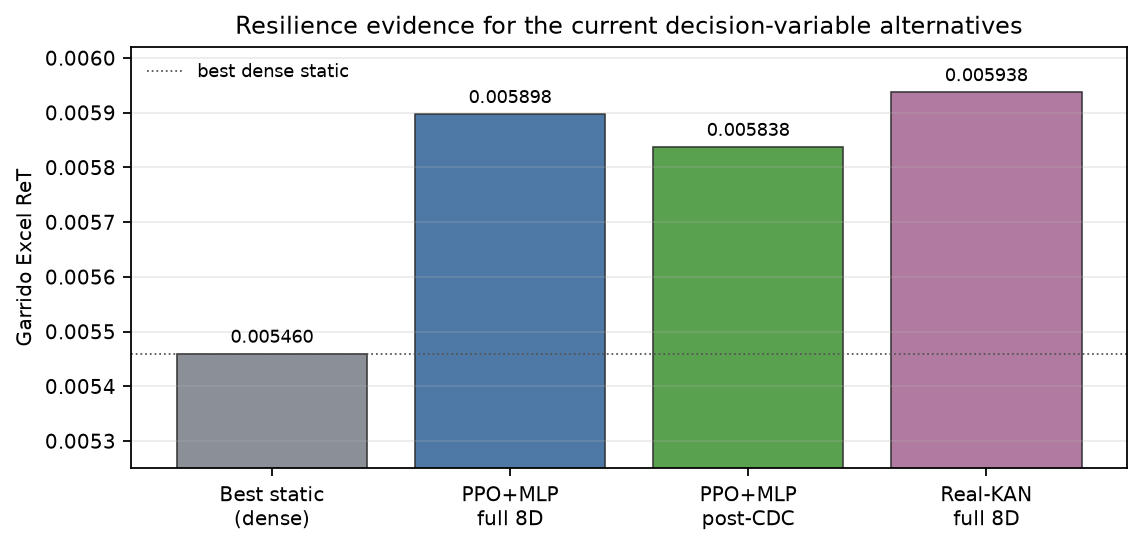
\includegraphics[width=0.82\linewidth]{figures/fig2_results_ret_bars.pdf}
  \caption{Excel ReT for the main evidence lanes.}
\end{figure}

\begin{figure}[ht]
  \centering
  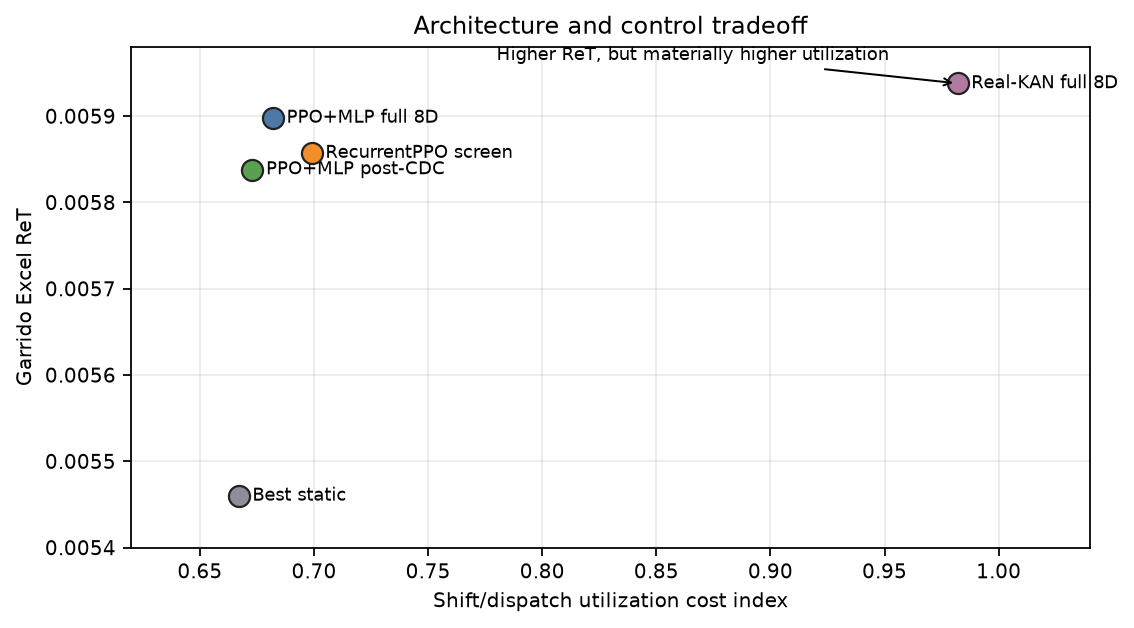
\includegraphics[width=0.82\linewidth]{figures/fig3_ret_cost_tradeoff.pdf}
  \caption{ReT-cost tradeoff. Real-KAN improves ReT, but at much higher utilization.}
\end{figure}

\begin{table}[ht]
\centering
\footnotesize
\begin{tabular}{p{0.30\linewidth}rrp{0.34\linewidth}}
\toprule
\textbf{Lane} & \textbf{Excel ReT} & \textbf{Delta} & \textbf{Interpretation} \\
\midrule
Best dense static & 0.005460 & -- & Strong non-learning baseline. \\
PPO+MLP full Track B & 0.005898 & +0.000438 & Main Paper 1 result; 10/10 seeds positive vs static. \\
PPO+MLP strict post-CDC & 0.005838 & +0.000410 & CDC control is not required; 5/5 seeds positive. \\
RecurrentPPO/LSTM & 0.005857 & +0.000406 & Memory alone beats static, but stays below PPO+MLP. \\
Real-KAN full Track B & 0.005938 & +0.000041 & Best ReT vs PPO+MLP; 10/10 positive, but high utilization cost. \\
\bottomrule
\end{tabular}
\caption{Evidence summary. Primary metric is Garrido/Excel ReT.}
\end{table}

\section*{What this says about learning capacity}

Both candidate directions show learning capacity:

\begin{itemize}[leftmargin=1.5em]
  \item \textbf{Track B operational control} already learns: PPO+MLP beats dense
  statics, heuristics, regime tables, masked-observation controls, and the
  strict post-CDC variant remains positive.
  \item \textbf{Architecture upgrades} also learn on Track B: RecurrentPPO beats
  static; DMLPA beats static but does not beat PPO+MLP; Real-KAN beats PPO+MLP
  on Excel ReT in 10/10 seeds.
  \item \textbf{Buffer-target control} is not yet proven as a learning lane. It
  is defensible if implemented conservatively, but should start with an oracle
  gate before a long CAN/KAN run.
\end{itemize}

\section*{Decision requested from Prof. Garrido}

We propose two viable routes:

\begin{enumerate}[leftmargin=1.5em]
  \item \textbf{Paper 1 conservative route:} use Track B operational dispatch
  variables as the main paper, with PPO+MLP as the clean baseline learner and
  Real-KAN as a confirmed architecture sidecar.
  \item \textbf{Garrido buffer route:} add conservative post-CDC buffer targets
  as a sidecar. If the static/oracle gate is positive, run a long CAN/KAN
  controller on that surface.
\end{enumerate}

Our recommendation is route 1 for the Q1 submission because it is already
statistically supported and physically conservative. Route 2 is the right way
to answer the literal buffer question, but it should not delay the current paper
unless Prof. Garrido prefers that scientific emphasis.

The final choice remains at Prof. Garrido's disposal. We can proceed with the
decision surface he considers most meaningful for the paper, provided the
replenishment mechanism remains physically conservative and the primary metric
remains the Garrido Excel resilience formula.

\end{document}
